%\subsubsection*{Las herramientas que adquieren datos}
El grado de avance que han experimentado la electrónica y la tecnología en general, gracias a la industria de los semiconductores, permite que la producción científica pueda adquirir una gran cantidad de datos. Para llevar a cabo la producción del conocimiento, es necesario el relevamiento y registro de diferentes tipos de magnitudes físicas y/o químicas sobre el objeto o proceso a investigar. En muchas ocasiones, estas magnitudes resultan difíciles de observar y cuantificar, por lo que es conveniente transformar las variables a conocer en otras más sencillas de medir. Para este propósito, se utilizan transductores.\\

Se conoce como transductor a cualquier dispositivo que recibe estímulos energéticos de una condición, situación o fenómeno físico y/o químico y los convierte en una señal asociada y definida de otra forma de energía\cite{Pallas-Areny2001,considine1971encyclopedia}. En otras palabras, los transductores son conversores de energías\cite{considine1971encyclopedia,Pallas-Areny2001,PerezGarcia2008}. Se denomina sensor a una clase particular de transductor que genera, como variable de salida, una señal eléctrica que está especialmente adaptada para ser ingresada en un circuito electrónico, o adecuada al sistema de medida que se utilice \cite{Fraden2010,Slawinski2011,Ogata2002}.\\

Las altas escalas de integración de circuitos alcanzadas en la actualidad posibilitan el diseño de sistemas sensoriales cada vez más complejos, en los cuales se logra agrupar miles de sensores en áreas reducidas, obteniendo medidas simultáneas y flujos crecientes de datos. Este trabajo se centrará en la transmisión de datos provenientes de sensores de imagen, uno de los desarrollos que se encuentra en boga.\\

Una imagen, desde un punto de vista digital, es un arreglo bidimensional de números, los cuales pueden ser exhibidos en una pantalla en forma de intensidad y colores de luz. Cada punto del arreglo que se muestra en pantalla se denomina pixel, acrónimo del ingles {\it PIcture ELement}, o elemento de imágen. Por esto, un sensor de imagen puede estar compuesto, bien por un arreglo bidimensional de sensores lumínicos (cómo la cámara de un teléfono celular), como por un transductor que es simultáneamente desplazado y medido, (método utilizado, entre otras, para la microscopía de fuerza atómica \cite{Binnig1983}), o por una combinación de ambos métodos. Por ejemplo, un scanner posee un arreglo lineal de transductores que son desplazados a través de la hoja para generar una imagen digital. En cualquiera de los casos, es de suma utilidad que la lectura de imágenes sea realizada en el menor tiempo posible, ya que cada imagen conlleva una cantidad no menor de datos.\\

\begin{figure}[t]
	\centering
	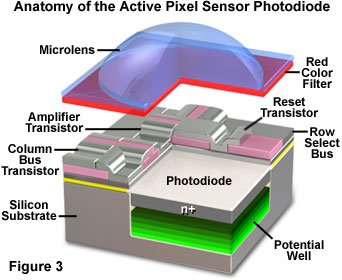
\includegraphics[width=0.43\textwidth]{aps-pixel}
	\caption{Esquema físico de un APS\cite{Turchetta2019}}
	\label{fig:pix}
\end{figure}

%TODO insertar aquí ejemplos de desarrollo de sensores de imágenes
Uno de los trabajos que más aportó al desarrollo de sensores de imágenes modernos, fue la introducción de los APS ({\it Active Pixel Sensor}, o sensor de pixeles activos) \cite{Mendis1994}. Este sensor integra en un proceso CMOS (acrónimo ingles de Metal-Óxido-Semiconductor Complementario, que es el método actualmente más económico para integrar transistores en una única pastilla de silicio), un fotodiodo, un transistor de reset (utilizado para controlar el tiempo de integración, es decir, de exposición a la luz) transistores de selección (utilizados para conectar un pixel determinado dentro del arreglo) y un amplificador seguidor de fuente en cada pixel\cite{Turchetta2019}. El fotodiodo, previamente cargado, transduce la luz en una descarga eléctrica y el amplificador convierte la carga remanente en tensión para facilitar su lectura. La Figura \ref{fig:pix} muestra el dibujo de un APS. Se observa el área sensible a la luz y los diferentes transistores que intervienen en su funcionamiento. Además se incorpora una micro-lente cuya función es la de enfocar los fotones sobre el área sensible y un filtro utilizado para identificar colores. En el caso de sensores monocromáticos, se omite la colocación del filtro de color durante la fabricación.\\

A partir del desarrollo de los APS, se fue perfeccionando el método hasta obtener circuitos integrados con mayor cantidad de pixeles y que pueden tener diversas aplicaciones. Por ejemplo, en los trabajos \cite{Hu-Guo2009} y \cite{Baudot2009} se presentan sensores CMOS basados en la arquitectura MIMOSA (de {\it Minimum Ionizing particule MOS Active pixel Sensor}%, Sensor con Pixel activo MOS de particulas ionizantes mínimas
). Estos sensores se desarrollaron con el objetivo específico de detección de radiación ionizante.\\

También existen desarrollos de sensores de radiación a través de APS comerciales. Perez {\it et al.} identificaron eventos producidos por partículas alfa en campos de radiación mixtos mediante el procesamiento de imágenes adquiridas con sensores comerciales CMOS\cite{Perez2016} y desarrollaron detectores de neutrones térmicos con sensores APS cubiertos con una capa de Gd$_2$O$_3$\cite{Perez2018Thermal}. Galimberti {\it et al.} utilizaron un sensor de imágenes comercial para realizar un detector de gas Rn en el ambiente\cite{Galimberti2018}. En otro trabajo, Hizawa, {\it et al.} fabricaron un sensor que adquiere imágenes midiendo el pH con cada uno de los pixeles\cite{Hizawa2007}, pudiendo observar de fenómenos químicos en tiempo real.\\

Como se mencionó antes, una imagen digital es un arreglo de datos. Esto quiere decir que un sensor de imágenes con $n$ pixeles de largo y $m$ de ancho, captura $n\times m$ datos en cada lectura. A su vez, para digitalizar valores, un circuito debe poseer, al menos, un conversor analógico-digital (ADC) de $x$ cantidad de bits, lo que implica que cada dato estará compuesto por $x$ dígitos binarios, es decir, un volumen importante de datos por cada lectura. Como ejemplo, un sensor comercial VGA, en su configuración más básica, posee 640 líneas horizontales y 480 verticales, con una resolución de 8 bits por cada pixel, lo que otorga 2.457.600 bits por cada lectura del sensor.\cite{ONSemiconductor2014} Si además se incorpora la cantidad de imágenes que se toman en función del tiempo (cuadros por segundo o fps), nos otorga un flujo de datos para nada despreciable.\\

Desde el punto de vista de la electrónica digital, para poder adquirir y transmitir grandes volúmenes de datos, se requiere de circuitos que sean capaces de operar a altas frecuencias de conmutación. El diseño de dichos circuitos no es trivial, ya que cuando las longitudes de onda de las señales presentes son comparables con las dimensiones físicas de dichos circuitos, debe considerarse el uso de líneas de transmisión\cite{Ida2015}. Esto implica que no se puede diseñar utilizando un criterio de uniformidad en los parámetros y exige un análisis mas detallado y preciso.\\
%se evidencian capacidades e inductancias parásitas que perjudican el desempeño de los sistemas. Las dimensiones son comparables cuando el largo del conductor es mayor a un cuarto de la longitud de onda de las señales que por él circulan. Por ejemplo, si se desea transmitir datos en serie a una frecuencia de \SI{300} {\mega\hertz}, la longitud de onda de la señal será de \SI{1}{\meter}.Esto quiere decir que  para este caso, \SI{25}{\centi\meter}. Si bien esto puede parecer grande, se debe notar que a mayores frecuencias, este efecto comienza a ser aún más perjudicial.\\

Otro problema que presentan los circuitos electrónicos digitales tiene que ver con los tiempos de propagación de las corrientes y tensiones que circulan a través de ellos. Cuando se aplica un impulso en un conductor, debido a las capacidades propias de los materiales utilizados, las tensiones pueden demorar unos instantes en establecerse. Puede suceder que varias señales lleguen a los puertos de un dispositivo por conductores con distintas longitudes y generen retardos diferentes. Esto puede ocasionar un comportamiento indeseado si no se toman los recaudos adecuados.\\

Aún suponiendo un perfecto diseño, los circuitos digitales de alta velocidad se encuentran limitados en la frecuencia de conmutación por la temperatura que se necesita disipar. La potencia consumida por estos dispositivos es proporcional a la frecuencia de funcionamiento\cite{Wakerly1999}. Parte de esta potencia se transforma en calor y produce un aumento en la temperatura. Si el incremento es indiscriminado, puede destruir los circuitos.\\

Una posible solución para disminuir la frecuencia de las señales sin perjudicar la tasa de transferencia es la incorporación de varios conductores para enviar datos en paralelo.
%Retornando al ejemplo de los datos transmitidos con variaciones de hasta \SI{300}{\mega\hertz}, si son enviados a través de dos conductores iguales, idénticos al anterior, la frecuencia necesaria cae a la mitad, con 3, se obtiene una reducción de la frecuencia a la tercera parte, con 10, es suficiente con un décimo, etc.
La cantidad de conductores a través de los cuales circula la información, se denomina ancho de bus. Idealmente, para lograr una tasa de transferencia determinada, se podría disminuir la frecuencia tantas veces cómo conductores se agreguen. Por ejemplo, transmitiendo por cuatro filamentos, se podría enviar la misma información a un cuarto de la frecuencia que se necesitaría con uno solo de iguales características.\\

Existen distintas tecnologías para efectuar la lectura de los datos generados por los sensores y su posterior transmisión. La incorporación y evolución de microcontroladores permite capturar y procesar volúmenes crecientes de datos. Sin embargo, este tipo de dispositivos posee una estructura rígida: su capacidad de procesamiento se encuentra limitada a una instrucción por ciclo de reloj y a un ancho de bus definido. Para aumentar los volúmenes de datos que circulan a través de ellos, no es posible aumentar el ancho de bus, sino que se torna necesario incrementar la frecuencia de funcionamiento, generando los problemas anteriormente detallados.\\

Una solución óptima, sin considerar los costos asociados a esto, sería el desarrollo de un circuito integrado de aplicación específica (ASIC del inglés {\it Application Specific Integrated Circuit}). En este tipo de circuitos, el diseñador elabora un circuito que puede operar a altas velocidades y, a su vez, obtener un ancho de bus sin restricciones, más que las dimensiones físicas del área donde será realizado el circuito. Sin embargo, cuando sí se considera el costo asociado a este enfoque, se vuelve una solución ineficiente en bajas cantidades. La manufactura de este tipo de dispositivos puede tener un costo de miles hasta cientos de miles de dólares, dependiendo del proceso de fabricación utilizado. Gran parte de estos costos son no recurrentes, es decir, solo se pagan una vez por proyecto. En grandes cantidades de dispositivos, este tipo de soluciones se vuelven más convenientes.\\

Otro enfoque, es la utilización de Arreglos de Compuertas Programables por Campo (FPGA, acrónimo del inglés {\it Field-Programmable Gate Array}). Un FPGA es un dispositivo electrónico que posee la capacidad de sintetizar casi cualquier circuito digital. En esencia, es una matriz de bloques lógicos (también llamadas {\it slices} o celdas lógicas, dependiendo del fabricante), que contienen Tablas de Verdad(LUTs o {\it Look-Up-Table}) y flip-flops (ff), entre otras cosas, y pueden ser interconectadas entre sí, según el criterio del usuario. Así, permite implementar una solución digital en un circuito físico, a diferencia de los microcontroladores, lo realiza a través de un algoritmo almacenado en una memoria, incorporando la ventaja de definir el ancho de bus necesario para relevar una gran cantidad de datos y transmitirlos a frecuencias de trabajo menores, además de ejecutar tareas en paralelo, disminuyendo los tiempos de procesamiento. A su vez, al ser implementado en un área muy pequeña, debido a la integración del sistema, este tipo de sistemas puede trabajar a frecuencias muy elevadas, lo que implica una mayor tasa de datos aún. A pesar de la gran diversidad de precios existentes en el mercado, una FPGA de costos menores a la centena de dólares suele tener muy buenas prestaciones para la mayor parte de las aplicaciones.\\

Existen diversas publicaciones en donde se observa el uso de FPGAs para la implementación de sistemas que producen imágenes. Por ejemplo, el desarrollo de un detector de radiación ionizante utilizando una sensor de imagen CMOS comercial. Para ello, los autores utilizaron una FPGA para configurar diversos parámetros del sensor con el fin de generar estrategias para la identificación de partículas alfa en campos de radiación mixtos y transmitir imágenes a una computadora personal (PC) a través de un puerto UART\cite{Perez2017}.
Se denomina ultrasonografía a la técnica de adquirir imágenes basandose en reflexiones de ultrasonido. Sus aplicaciones son múltiples, en las que se destaca el diagnóstico médico debido. Un trabajo reciente desarrolló un sistema que mejora la obtención de ecografías médicas con bajo costo utilizando una FPGA\cite{biswas2018embedded}. El autor presentó un algoritmo para la supresión de ruido de impulso en tiempo real para imágenes codificadas como JPEG 2000 realizado y probado en Matlab e implementado en una FPGA.
Yanagisawa {\it et al}, desarrollaron un sistema con telescopios pequeños para explorar objetos de campo cercano con la finalidad de monitorear cuerpos celestes que puedan colisionar con el planeta\cite{Yanagisawa2018}. En este trabajo, se aprovechó la velocidad de los circuitos implementados en FPGA para minimizar el tiempo de adquisición.\\

El desarrollo de nuevos sensores brinda a los investigadores un gran volumen de datos. En muchos casos, la obtención de datos por si misma no otorga información, sino que es necesario procesar y analizar los mismos. La invención y evolución de las computadoras, como así también el desarrollo de nuevos algoritmos, dan lugar a procesamiento de datos cada vez más complejos en tiempos mucho menores.
Las primeras ENIAC, computadoras de propósito general desarrollada en el año 1946 para el cálculo de tablas balísticas de las fuerzas armadas estadounidenses, podía ejecutar 20 operaciones cada \SI{10}{\micro\second} \cite{Goldstine1946}, es decir, ejecutaba instrucciones con una frecuencia máxima de \SI{200}{\kilo\hertz}. A su vez, tuvo un costo aproximado de U\$S 500.000, pesaba 5 t y consumía \SI{175}{\kilo\watt}.
En contraste con aquello, es posible conseguir en el mercado actual, computadoras con tamaño y peso reducido, que ejecutan instrucciones en cuenstión de nanosegundos, (5 ordenes de magnitud menos), consumen menos de \SI{1}{\kilo\watt} y cuestan algunos cientos de U\$S. A tal punto ha evolucionado esta tecnología, que se cuenta con computadoras muy potentes en casi cualquier laboratorio, oficina u hogar. La capacidad de cálculo que exhiben estos dispositivos, sumada al desarrollo de nuevos métodos y algoritmos de cálculo, permite a los investigadores procesar datos en tiempo reducido, facilitando el análisis y la generación de nueva información.\\

En todos los casos que se consideran en este trabajo, la generación de datos y el procesamiento de lo mismos se da en sistemas diferentes. Es decir, los datos son relevados por los sensores y adquiridos luego por los FPGAs. Finalmente llegan a una PC para su posterior procesamiento y análisis. Se requiere, por tanto, de una conexión a través de la cual los datos puedan ser transferidos del sistema de adquisición, la FPGA, a la PC y viceversa. Se torna de suma utilidad, entonces, proveer una comunicación efectiva y robusta que permita transmitir grandes volúmenes de datos en poco tiempo, y de esta forma facilitar los tiempos de desarrollo, pruebas, depuración, procesamiento y análisis.\\

%Desde un punto de vista electrónico, para poder transmitir gzrandes volúmenes de datos en forma digital, se requiere de circuitos que sean capaces de operar a altas frecuencias de conmutación. Esto no es trivial, ya que cuando las longitudes de onda que se mueven a través de un circuito son comparables con sus dimensiones físicas, se evidencian capacidades e inductancias parásitas no contempladas que perjudican el desempeño de los sistemas. Por ejemplo, si se desea transmitir datos en serie con una variación entre sus datos de \SI{300} {\mega\hertz}, se habla de ondas cuya longitud de onda es de \SI{1}{\meter}. Se dice que las dimensiones son comparables cuando el largo del conductor posee al menos un cuarto de la longitud de onda, es decir, para este caso, \SI{25}{\centi\meter}. Si bien esto puede parecer grande, se debe notar que a mayores frecuencias, este efecto comienza a ser aún más perjudicial.\\
%
%Otro problema que presentan los circuitos de alta velocidad tiene que ver con los tiempos de propagación de las corrientes y tensiones que circulan a través de ellos. Cuando se aplica un impulso en un conductor, la onda viaja a la velocidad de la luz. Esto quiere decir que la tensión no llega al mismo tiempo a todos los puntos del circuito, sino que, mientras más alejada está la fuente, más lejos está se demora en responder. Puede suceder, entonces, que la lógica del circuito se demore más que el pulso de reloj que indica un cambio de estado, obteniendo así un comportamiento no deseado, si no está correctamente diseñado y contemplado este aspecto.\\
%
%Una solución para los circuitos electrónicos que necesitan mover grandes volúmenes de datos, puede ser la incorporación varios conductores a través de los cuales puede fluir la información. Retornando al ejemplo de los datos transmitidos con variaciones de hasta \SI{300}{\mega\hertz}, si son enviados a través de dos conductores iguales, idénticos al anterior, la frecuencia necesaria cae sería la mitad, con 3, se obtiene una reducción de la frecuencia a la tercera parte, con 10, es suficiente con un décimo, etc. La cantidad de conductores a través de los cuales circula la información, se denomina ancho de bus.\\
%
%En gran medida, la incorporación y evolución de microcontroladores permite capturar y procesar volúmenes crecientes de datos. Sin embargo, este tipo de dispositivos posee una estructura rígida, capacidad de procesamiento limitada a una instrucción por vez y ancho de bus definido, la única opción para aumentar los volúmenes de datos que circulan a través de ellos, es un aumento de la frecuencia de funcionamiento, generando los problemas anteriormente detallados.\\
%
%Una solución óptima, sin considerar los costos asociados a esto, sería el desarrollo de un circuito integrado de aplicación específica (ASIC del inglés {\it Application Specific Integrated Circuit}). En este tipo de circuitos, el diseñador elabora un circuito que puede operar a altas velocidades y, a su vez, obtener un ancho de bus sin restricciones, más que las dimensiones físicas del área donde será realizado el circuito. Sin embargo, cuando sí se considera el costo asociado a este enfoque, se vuelve una solución ineficiente en bajas cantidades. La manufactura de este tipo de dispositivos puede tener un costo de miles hasta cientos de miles de dólares, dependiendo del proceso de fabricación utilizado. Gran parte de estos costos son no recurrentes, es decir, solo se pagan una vez por proyecto. En grandes cantidades de dispositivos, este tipo de soluciones se vuelven más convenientes.\\
%
%Otro enfoque, es la utilización de Arreglos de Compuertas Programables por Campo (FPGA, acrónimo del inglés {\it Field-Programmable Gate Array}). Un FPGA es un dispositivo electrónico que posee la capacidad de sintetizar casi cualquier circuito digital. En esencia, es una matriz de bloques lógicos (también llamadas {\it slices} o celdas lógicas, dependiendo del fabricante), que contienen Tablas de Verdad(LUTs o {\it Look-Up-Table}) y flip-flops (ff), entre otras cosas, y pueden ser interconectadas entre sí, según el criterio del usuario. Así, permite implementar una solución digital en un circuito físico, a diferencia del microcontrolador que lo realiza a través de un algoritmo almacenado en una memoria, incorporando la ventaja de definir el ancho de bus necesario para relevar una gran cantidad de datos y transmitirlos a frecuencias de trabajo menores, además de ejecutar tareas en paralelo, disminuyendo los tiempos de procesamiento. A su vez, al ser implementado en un área muy pequeña, debido a la integración del sistema, este tipo de sistemas puede trabajar a frecuencias muy elevadas, lo que implica una mayor tasa de datos aún. A pesar de la gran diversidad de precios existentes en el mercado, una FPGA de costos menores a la centena de dólares suele tener muy buenas prestaciones para la mayor parte de las aplicaciones.\\
%
%Existen diversas publicaciones en donde se observa el uso de FPGAs para la implementación de sistemas que producen imágenes. Por ejemplo, el desarrollo de un detector de radiación ionizante utilizando una sensor CMOS comercial. Para ello, los autores utilizaron una FPGA para configurar diversos parámetros del sensor y transmitir imágenes a una computadora personal (PC) a través de un puerto UART. Esto permitió adquirir una imagen accionando un disparador realizado con un pulsador\cite{Perez2017}.\\
%
%Se denomina ultrasonografía a la técnica de adquirir imágenes basandose en reflexiones de ultrasonido. Sus aplicaciones son múltiples, en las que se destaca el diagnóstico médico debido. Un trabajo reciente desarrolló un sistema de ecografía médica con bajo costo utilizando una FPGA\cite{biswas2018embedded}. El autor también presentó un algoritmo realizado y probado en PC. Luego se implementó e en una FPGA.\\
%
%Yanagisawa {\it et al}, desarrollaron un sistema con telescopios pequeños para explorar objetos de campo cercano con la finalidad de monitorear cuerpos celestes que puedan colisionar con el planeta\cite{Yanagisawa2018}. En este trabajo, se aprovechó la velocidad de los circuitos implementados en FPGA para minimizar el tiempo de adquisición.\\

La implementación de un sistema de comunicación en una FPGA puede ser resuelta de muchas maneras, quedando a criterio del desarrollador utilizar algún protocolo estándar, o bien diseñar uno propio. Sin embargo, en una computadora, las formas de comunicar datos se vuelven un poco más restrictivas y acotadas a los puertos y señales que puede manejar el equipo, conforme el fabricante haya establecido.
Este trabajo busca implementar una comunicación entre una computadora personal y una FPGA, utilizando un protocolo estándar, que esté disponible en cualquier computadora comercial y que posea una tasa de bit suficiente para poder transmitir imágenes.\\


%Es por esto que la PC {\it Personal Computer} se ha transformado en la herramienta indispensable en cualquier ámbito, pero en especial en los entornos en donde se requiere el  manejo, cálculo, procesamiento y análisis de grandes cantidades de datos e información.\\
%
%
%
%Desde la inclusión de la norma USB, en el año 1996 a la fecha, se ha convertido en el elemento que no falta en ningun equipo, al punto tal que ha desplazado a cualquier otro conector. Al punto tal es esto, que para requerir algún puerto adicional que no sea de esta norma, cualquier comprador debe especificar que así sea, mas no es necesario especificar que tiene USB como norma de conexión.\\
%
%El presente trabajo pretende ofrecer una comunicación basada en la versión 2.0 de la norma USB entre una PC y un FPGA, y otorgue una herramienta adicional a científicos que desarrollen o utilicen sistemas basados en FPGA.\\
%
%Este trabajo, pretende elaborar una interfaz entre los dos extremos, es decir, entre la PFGA y la PC, de forma tal que permita a un desarrollador, investigador o usuario en general, obtener una comunicación confiable y con un ancho de banda que permita mover el flujo de datos que genera una sensor que adquiera imágenes.\\
%
%Es cierto que el protocolo puede ser totalmente implementado en una FPGA, sin embargo, esto requeriría un muy alto costo tanto económico como en recursos disponibles del chip programable para una tarea genérica que es mejor elaborar con un circuito integrado diseñado especialmente para tal fin. Es por esto que se utiliza como lazo de interfaz un chip comercial elaborado por Cypress Semiconductor.\\
%
%
%
%[1][https://ieeexplore.ieee.org/abstract/document/8214376]
%[2][http://www.idr.iitkgp.ac.in/jspui/bitstream/123456789/9068/1/NB15975_Abstract.pdf]
%[3][https://ieeexplore.ieee.org/abstract/document/8396725]




%El mundo actual, en el que vivimos inmersos, demanda y consume volumenes cada vez más grandes de información. Con solo hacer una rapida miradad en diarios, incluso no especilizados, se observa la importancia que poseen las ciencias y disciplinas que manejas la informacion, aquellas areas agrupadas dentro del conjunto Técnico de la Información y la Comunicación, o más ocnocido por sus siglas, TIC's.
%
%Internet de las cosas , Big Data, Inteligencia Artificial, Redes Neuronales, Robótica, Domótica, entre otras, son areas en las que los datos y la información es abultada y su correcto manejo es sumamente complejo e importante. Además, ninguna de las actividades científicas, puede escapar de esta gran demanda mundial de información.
%
%La información es un conjunto de datos ordenados y procesados de forma tal que permita al que lo lea que eleve su nivel de conocimiento sobre un determinado tema. Es decir que, para que exista información, en primer lugar tenemos que tener datos, de forma tal que podamos luego procesarlos y obtener realmente información de llos.
%
%Como ejemplo de esto, podemos citar simplemente el acto de medir la presión dentro de un tubo de gas. Sería normal pensar en que, teniendo este objetivo en mente, simplemente coloquemos un manómetro en la salida del tubo. El manómetro es un artefacto que posee una varilla 
%
%
%
%
%
%El mundo, durante la era de la información, nos exige producir y consumir cada vez más y más información. En cada aspecto social dela vida de la persona se pueden encontrar ejemplos claros de esto.\\
%
%Bajo un punto de vista social nos vemos bombardeados por información. Los 'influencers' que se mueven a traves de Facebook, Twiter, Instagram, Snapchat, Linkedin, Youtube, etc, necesitan para estar a la moda, producir constantemente material y que ese material sea consumido por alguien que este demandando esa información.
%
%En el area de econimía y finanzas existen cada vez más robots que extraen información de las diferentes bolsas, periodicos, bancos, industrias y donde se ocurra que pueda haber información útil, para tomar mejores decisiones que, por supuesto, también ejecutan los robots.
%
%En el comercio, desde las tiendas de supermercado hasta las tiendas digitales que trabajan solo a través de internet están constantemente recabando datos y procesandolos a din de diseñar estrategias que permitan ofrecer productos que se adapten mejor a lo que busca el cliente y de esa forma lograr vender mayores volumenes.
%
%La industria cuenta cada vez más con multiplicidad de posibilidades basadas en sensores que adquieren grandes cantidades de datos que son almacenadas y procesadas, muchas vecen 'en línea' o 'al instante', de forma tal de encontrar mejores procesos o ejecutar nuevas tareas, como por ejemplo la industria automotriz, enfocada cada vez más en autos que puedan manipular todo el entorno y ser totalmente autónomos de un conductor.
%La industria espacial y satelital dotan a sus equipos de mayores sensores y mayores flujos de datos. La industria médica brinda cada vez más posibilidades de diagnóstico a traves de nuevas técnicas y formas de adquisición de imágenes.
%
%A todo esto, la ciencia y el desarrollo de nuevas aplicaciones y equipos, no son indiferente. Cada vez se encuentran más innovaciones y desarrollos de nuevos sensores que adquieren flujos de información crecientes. La toma de imagenes se ha vuelto una herramienta clave para la investigación en diversas areas, tales como la biología, la ciencia de materiales, las ciencias nucleares, las ciencias de la tierra, etc.
%
%Las redes sociales son un ejemplo de esto, pero esto se observa en la industria, la economía, las finanzas e incluso hasta en la casa.
%
%
%
%[1] file:///home/lechuzin/Facultad/Trabajo%20Final/lechuzing/docs/bibliografia/The-Rise-of-the-Network-Society-With-a-New-Preface-Volume-I-The-Information-Age-Economy-Society-and-Culture-Information-Age-Series-.pdf